\newpage
\chapter{\textbf{Dynamic Programming}}
Dynamic Programming is mainly an optimization over plain recursion. Wherever we see a recursive solution that has repeated calls for same inputs, we can optimize it using Dynamic Programming. The idea is to simply store the results of subproblems, so that we do not have to re-compute them when needed later. This simple optimization reduces time complexities from exponential to polynomial.

\section{\textbf{Travel at Minimum Coast}}

\begin{center}
	\begin{tabular}{c  c  c}
		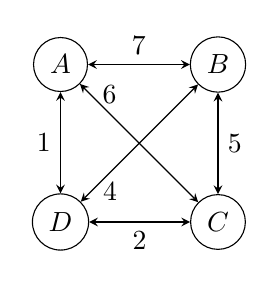
\begin{tikzpicture}
		
		\node[draw, circle, minimum size=0.6cm] (nodeA) at (-2,0){$A$};
		\node[draw, circle, minimum size=0.6cm] (nodeB) at (0,0){$B$};
		\node[draw, circle, minimum size=0.6cm] (nodeC) at (0,-2){$C$};
		\node[draw, circle, minimum size=0.6cm] (nodeD) at (-2,-2){$D$};
		
		%%%%% Arrows %%%%%%
		\draw[stealth-stealth] (nodeA)--(nodeB)node[midway,above]{$7$};
		\draw[stealth-stealth] (nodeB)--(nodeC)node[midway,right]{$5$};	
		\draw[stealth-stealth] (nodeC)--(nodeD)node[midway,below]{$2$};
		\draw[stealth-stealth] (nodeD)--(nodeA)node[midway,left]{$1$};
		\draw[stealth-stealth] (nodeA)--(nodeC)node[near start,above]{$6$};
		\draw[stealth-stealth] (nodeB)--(nodeD)node[near end,below]{$4$};	
		
		\end{tikzpicture}
		
		&
		
		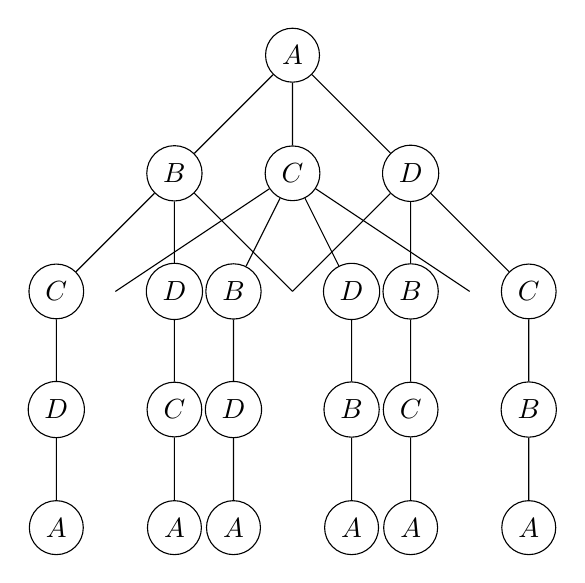
\begin{tikzpicture}
		
		\node[draw, circle, minimum size=0.6] at (0,0){$A$}
			child { 
				node[draw, circle, minimum size=0.6]{$B$}
				child {
					node[draw, circle, minimum size=0.6]{$C$}
					child {
						node[draw, circle, minimum size=0.6]{$D$}
						child {node[draw, circle, minimum size=0.6]{$A$}}
					}
				}
				child {
					node[draw, circle, minimum size=0.6]{$D$}
					child {
						node[draw, circle, minimum size=0.6]{$C$}
						child {node[draw, circle, minimum size=0.6]{$A$}}
					}
				}
				child{}
			}		
			child { 
				node[draw, circle, minimum size=0.6]{$C$}
				child{}
				child {
					node[draw, circle, minimum size=0.6]{$B$}
					child {
						node[draw, circle, minimum size=0.6]{$D$}
						child {node[draw, circle, minimum size=0.6]{$A$}}
					}
				}
				child {
					node[draw, circle, minimum size=0.6]{$D$}
					child {
						node[draw, circle, minimum size=0.6]{$B$}
						child {node[draw, circle, minimum size=0.6]{$A$}}
					}
				}
				child{}
			}
			child { 
				node[draw, circle, minimum size=0.6]{$D$}
				child{}
				child {
					node[draw, circle, minimum size=0.6]{$B$}
					child {
						node[draw, circle, minimum size=0.6]{$C$}
						child {node[draw, circle, minimum size=0.6]{$A$}}
					}
				}
				child {
					node[draw, circle, minimum size=0.6]{$C$}
					child {
						node[draw, circle, minimum size=0.6]{$B$}
						child {node[draw, circle, minimum size=0.6]{$A$}}
					}
				}
			}
			
			;
		\end{tikzpicture}
		
		&
		
		\begin{blockarray}{ccccc}
		& A & B & C & D \\
		\begin{block}{c[cccc]}
		A & 0 & 7 & 6 & 1 \\
		B & 7 & 0 & 5 & 4 \\
		C & 6 & 5 & 0 & 2 \\
		D & 1 & 4 & 2 & 0 \\
		\end{block}
		\end{blockarray}
		
	
	\end{tabular}
\end{center}

%%%%%%%%%%%%%%% Recursive Solution %%%%%%%%%%%%%%%%%%%%%
\newpage
\subsection{Recursive Solution}

\begin{lstlisting}[language=C++]
#include<bits/stdc++.h>
using namespace std;

int tsp(vector<vector<int>>dist, int setOfCities, int currentCity, int numberOfCities) {
    // Check if all the cities are visited
    if(setOfCities==(1<<numberOfCities)-1) {
        // return the cost to visit from last note to start node
        return dist[currentCity][0]; 
    }

    int ans = INT_MAX;

    for(int nextCity=1; nextCity<numberOfCities; nextCity++) {
        // Check if the current city is visited or not
        if((setOfCities & (1<<nextCity)) == 0) {  
            int cost = dist[currentCity][nextCity];
            // Update the visited cities status
            int update = (setOfCities | (1<<nextCity));
            cost += tsp(dist, update, nextCity, numberOfCities);
            ans = min(ans,cost);
        }
    }

    return ans;
}

int main() {
    vector < vector<int>> dist;
    dist = {
        {0,7,6,1},
        {7,0,5,4},
        {6,5,0,2},
        {1,4,2,0}
    };
    int numberOfCities = 4;
    cout << tsp(dist,1,0,numberOfCities) << endl;

    return 0;
}
\end{lstlisting}

%%%%%%%%%%%%%%%%%%%%%% DP Solution %%%%%%%%%%%%%%%%%
\newpage
\subsection{DP Based Solution}

\begin{lstlisting}[language=C++]
#include<bits/stdc++.h>
using namespace std;

int tsp(vector<vector<int>>dist, int setOfCities, int crntCT, int numOfCTs, vector<vector<int>>dp) {
    // Check if all the cities are visited
    if(setOfCities==(1<<numOfCTs)-1) 
        return dist[crntCT][0]; // cost to visit last to start

    if(dp[setOfCities][crntCT] != -1) // check if current is visited
        return dp[setOfCities][crntCT];

    int ans = INT_MAX;
    for(int nxtCT=1; nxtCT<numOfCTs; nxtCT++) {
        if((setOfCities & (1<<nxtCT)) == 0) {  
            int update = (setOfCities | (1<<nxtCT));
            int cost = dist[crntCT][nxtCT] + tsp(dist, update, nxtCT, numOfCTs,dp);
            ans = min(ans,cost);
        }
    }
    dp[setOfCities][crntCT] = ans; // Memorise visited city cost
    return ans;
}

int main() {
    vector < vector<int>> dist;
    dist = {
        {0,5,7,3},
        {2,0,4,2},
        {5,2,0,3},
        {4,2,3,0}
    };
    int numOfCTs = 4;
    vector < vector<int>> dp(1<<numOfCTs, vector<int>(numOfCTs,-1));
    cout << tsp(dist,1,0,numOfCTs,dp) << endl;
    return 0;
}
\end{lstlisting}
		

